\chapter{Предлагаемый метод для мультипликативных неопределённостей}\label{ch:ch3}
\section{Линеаризация}\label{sec:ch3/sect1}
Конфигурация шагающего робота может быть описана вектором обобщённых координат $q$. Обобщённые координаты и их производные $\dot q$ вместе образуют вектор состояния робота $x$. Взаимодействие робота с окружающей средой можно описать как ограничение на скорость изменения состояния \cite{mason2014full}: ${G} \dot x = 0$. Это мотивирует ортогональную декомпозицию вектора состояния:
%
\begin{equation}
	x = {N} z^* + {R} \zeta^* ,
\end{equation}
%
где $z^*$ --- координаты состояния, изменяющиеся со временем, а $\zeta^* = \text{const}$, матрицы ${N}$ и ${R}$ --- ортонормированные базисы в подпространстве нулей и подпространстве строк матрицы ограничений ${G}$.

Рассмотрим уравнение динамики $\dot z^* = f(z^*, \zeta^*)$ с параметрами $\zeta^* = \text{const}$ и его разложение Тейлора в окрестности точки $z^* = z_0$, $\zeta^* = \zeta_0$. Определим $z = z^* - z_0$ и $\zeta = \zeta^* - \zeta_0$.
Опустив квадратичные члены и члены высших порядков, но сохранив линейные и билинейные члены, запишем приближенную динамику в виде:
%
\begin{equation}
	\label{eq:model_linearization_1}
	\dot z = \frac{\partial f}{\partial z} z + \Delta {A}(\zeta) z + \frac{\partial f}{\partial \zeta} \zeta ,
\end{equation}
%
где $\Delta {A}(\zeta) = \frac{\partial}{\partial z} (\frac{\partial f}{\partial \zeta} \zeta)$. Мы оставляем билинейный член $\Delta {A}(\zeta) z$ потому, что $\zeta$ постоянна, а $\Delta {A}(\zeta)$ не обращается в нуль и влияет на устойчивость системы.

Модель \eqref{eq:model_linearization_1} включает в себя как мультипликативные, так и аддитивные неопределённости. Мы можем интерпретировать постоянные параметры $\zeta$ как неопределённые параметры модели, либо как статические компоненты состояния шагающего робота. В последнем случае мы приходим к модели шагающего робота на временном интервале между последовательными шагами.

Предположим, что основным источником неопределённости в рассматриваемой динамике является геометрия окружающей среды (опорной поверхности), с которой соприкасается робот. Пусть $K_s$ --- точка на опорной поверхности, а $K_r$ --- точка на теле робота, которая с ней соприкасается (т. е. точка на ноге робота). Пусть $e_K$ --- вектор нормали к опорной поверхности в точке $K_s$, а $h_K(q) \in \mathbb{R}$ --- вектор, проведённый из $K_r$ в $K_s$, спроецированный на $e_k$. Тогда мы можем моделировать неопределённость как:
%
\begin{equation}
	\label{eq:uncertain_contact}
	h_K(q) = \Delta h,
\end{equation}
%
где $\Delta h$ --- неточность в положении точки $K_s$. Если робот соприкасается с опорной поверхностью, это означает, что конфигурация робота описывается не координатами $q$, а $q + \Delta q$, где $\Delta q$ --- неточность конфигурации. Мы можем определить несоответствие состояния как 
$\Delta x = \begin{bmatrix}
	\Delta q \\ \Delta \dot q
\end{bmatrix}$
и находим, что связь между статическими состояниями и неточностью состояний имеет вид $\zeta = {R}\T \Delta x$. Написав разложение Тейлора для \eqref{eq:uncertain_contact} и его производной, находим:
%
\begin{align} 
	\label{eq:J_Delta_q} 
	{J}_K \Delta q = \Delta h,
	\\
	\label{eq:J_Delta_qdot} 
	{J}_K \Delta \dot q + \dot{{J}}_K \Delta q = \Delta \dot h,
\end{align}
%
где ${J}_K = \partial h_K / \partial q$.
Предположим, что $\Delta \dot h = 0$ и $\Delta h$ --- неизвестная скалярная переменная с областью определения $-s_K \leq \Delta h \leq s_K$, где $s_K$ --- положительный скаляр. Тогда мы можем вычислить расхождение состояний как решение по методу наименьших квадратов для \eqref{eq:J_Delta_q} и\eqref{eq:J_Delta_qdot}. Проецируя это решение на столбцы $R$, находим $\zeta$:
%
\begin{align}
	\zeta = {R}\T 
	\begin{bmatrix}
		{J}_K & 0 \\ \dot{{J}}_K & {J}_K
	\end{bmatrix}^+ 
	\begin{bmatrix}
		s_K \\ 0
	\end{bmatrix} \varsigma,
\end{align}
%
где $-1 \leq \varsigma \leq 1$. Учитывая определение $\Delta {A}(\zeta)$, мы можем написать:
\begin{equation}
	\Delta {A}(\zeta) = 
	\frac{\partial}{\partial z} 
	\left (
	\frac{\partial f}{\partial \zeta} {R}\T 
	\begin{bmatrix}
		{J}_K & 0 \\ \dot{{J}}_K & {J}_K
	\end{bmatrix}^+ 
	\begin{bmatrix}
		s_K \\ 0
	\end{bmatrix} \varsigma 
	\right )
	= \Tilde{A} \varsigma,
\end{equation}
%
где $\Tilde{A}$ --- некоторая матрица, образующая базис в пространстве допустимых значений неопределённой матрицы $\Delta {A}$.

Наша цель --- получить такие матрицы ${M}_1$, ${F}_1$ и ${N}_1$, где ${F}_1\T {F}_1 \leq {I}$, что для любого выбранного вектора $z$ множество всех векторов ${M}_1 {F}_1 {N}_1 z$ будет содержать множество $(\Tilde{A} \varsigma) z$. Учитывая сингулярное разложение $\Tilde{A} = {U}_A {\Sigma}_A {N}_1\T$, где 
${U}_A = \begin{bmatrix}
	{u}_1, ..., {u}_n
\end{bmatrix}$, 
${\Sigma}_A = \text{diag}(\sigma_1, ..., \sigma_n)$, мы определяем новую матрицу ${M}_1$:
%
\begin{equation}
	{M}_1 = 
	\begin{bmatrix}
		\sigma_1{u}_1, ..., \sigma_n{u}_n
	\end{bmatrix}.
\end{equation}
Таким образом, мы можем описать матрицу эквивалентным образом $\Delta {A} = {M}_1 {F}_1 {N}_1$, где ${F}_1\T{F}_1\leq {I}$.

\section{Мультипликативные неопределённости}\label{sec:ch3/sect2}

В этом разделе мы рассматриваем формулировку системы описывающей динамику шагающего робота, в которой мультипликативные неопределённости накладываются на каждую из матриц модели. Наша цель --- предоставить новые методы для проектирования робастного управления, а также показать дополнительную устойчивость к неопределённости, которая может быть достигнута при отмене влияния статической части состояния.

Рассмотрим следующую систему: 
%
\begin{equation}
	\label{eq:part2_linear_dynamics}
	\begin{cases}
		\dot z=({A}_n+\Delta {A}_n)z + ({B}+\Delta {B})u,\\
		y = ({C}+ \Delta {C}){N}  z,
	\end{cases}
\end{equation}
%
где $A_n \in \mathbb{R}^{n_z \times n_z}$ --- матрица состояния, $B \in \mathbb{R}^{n_z \times m}$ --- матрица управления, $C \in \mathbb{R}^{l \times n}$ --- матрица наблюдения, а неопределённые матрицы состояния, управления и наблюдения определяются как:
%
\begin{equation}
	\label{eq:part2_uncertainty}
	\Delta {A}_n={M}_1{F}_1{N}_1, \ \ \Delta {B}= {M}_2{F}_2{N}_2, \ \
	\Delta {C} = {M}_3{F}_3{N}_3; 
\end{equation}
%
где ${M}_1 \in \mathbb{R}^{n_z \times d}$, 
${N}_1 \in \mathbb{R}^{d \times n_z}$ , ${M}_2 \in \mathbb{R}^{n_z \times p}$,
${N}_2 \in \mathbb{R}^{p \times m}$, ${M}_3 \in \mathbb{R}^{l \times q}$,
${N}_3 \in \mathbb{R}^{q \times n}$ --- известные матрицы, 
а ${F}_i$ --- неизвестные матрицы ограниченные по норме ${F}_i\T{F}_i\leq \nu_i {I}$, где $\nu_i$ --- радиусы неопределённости --- скаляры, определяющие ограничения, накладываемые на нормы ${F}_i$. 

Следуя \cite{SAVIN2021}, для получения оценки вектора состояния, вводим наблюдатель Люенбергера с состоянием $\hat{z}$:
%
\begin{equation}
	\label{eq:Luenberger}
	\dot{\hat{z}}={A}_n\hat{z}+{B}u+{L}_z(y- {C} {N}\hat{z}),
\end{equation}
%
где ${L}_z$ --- матрица наблюдателя, обеспечивающая требуемый вид переходных процессов оценки вектора состояния. 
 
Введём ошибку восстановления $e_z=z-\hat{z}$, и запишем ошибку восстановления для динамики:
%
\begin{equation}
	\label{eq:part2_error_dynamics}
	\dot{e}_z=({A}_n-{L}_z{C}{N}) e_z +(\Delta {A}_n -{L}_z\Delta {C}{N}) z +\Delta {B} u.
\end{equation}
%
Рассмотрим следующий закон управления с линейной обратной связью:
%
\begin{equation}
	\label{eq:control_law}
	u={K}_z\hat{z}.
\end{equation}
%
Подставим закон управления \eqref{eq:control_law} в уравнение \eqref{eq:Luenberger}:
\begin{equation}
	\label{eq:Luenberger_K}
	\dot{\hat{z}}={A}_n\hat{z}+{B}K_z \hat{z} +{L}_z C N z +{L}_z \Delta C N z- {L}_z {C} {N}\hat{z}),
\end{equation}
и подставим закон управления \eqref{eq:control_law} в ошибку восстановления для динамики \eqref{eq:part2_error_dynamics}:
%
\begin{equation}
	\label{eq:error_dynamics_K}
	\dot{e}_z=({A}_n-{L}_z{C}{N}) e_z +(\Delta {A}_n -{L}_z\Delta {C}{N}) z +\Delta {B} K_z \hat{z}.
\end{equation}
%
Введём новый вектор состояния, объединив предыдущий вектор состояния и ошибку восстановления $ \begin{bmatrix}
	z \\ e_z
\end{bmatrix}$, при этом динамика принимает вид:
%
\begin{equation}
	\label{eq:part2_system}
	\begin{bmatrix}
		\dot{z} \\ \dot{e}_z
	\end{bmatrix}=\begin{bmatrix}
		({A}_n+\Delta {A}_n +{B}{K}_z+\Delta {B}{K}_z) & -({B}{K}_z+\Delta {B}{K}_z) \\
		(\Delta {A}_n +\Delta {B}{K}_z-{L}_z\Delta {C}{N}) & ({A}_n-{L}_z{C}{N}-\Delta {B}{K}_z)        \end{bmatrix}\begin{bmatrix}
		z \\ e_z
	\end{bmatrix}.
\end{equation}

В этом подразделе мы рассмотрим случай, когда радиус неопределённости равен $\nu_i = 1$, поэтому границы неопределённости определяются как:
%
\begin{equation}
	\label{eq:part2_one_uncertainty}
	{F}_i\T{F}_i\leq {I}, \ \ i=1,2,3.
\end{equation}
%
\begin{theorem}\label{thm:part2_LMI_1}
	Система \eqref{eq:part2_system} асимптотически устойчива при любом выборе $\Delta {A}_n$, $\Delta {B}$, $\Delta {C}$, удовлетворяющих условиям \eqref{eq:part2_uncertainty} и \eqref{eq:part2_one_uncertainty}, если существуют положительно--определённые матрицы ${Q}_1>0$, ${P}_2>0$, матрицы $\hat{{K}}$, $\hat{{L}}$,
	и положительные скаляры $\alpha_1>0, \beta_1>0, \alpha_2>0, \beta_2>0, \alpha_3>0, \beta_3>0$ и $\epsilon_1 > 0$ такие, что выполняется следующее линейно--матричное неравенство:
	%
	\begin{equation}
		\label{eq:thm3_final_LMI}
		\begin{bmatrix}
			\mathcal{T}_{11} & \mathcal{T}_{12} \\
			* & \mathcal{T}_{22}
		\end{bmatrix}<0,
	\end{equation}
	%
	где
	%
	\begin{equation}
		\mathcal{T}_{11}= \begin{bmatrix}
			{\Lambda}_1 & 0 & {M}_1 & {M}_2&0 & {Q}_1{N}_1\T & \hat{{K}}_z\T{N}_2\T & {Q}_1 {N}\T{N}_3\T \\
			* & {\Lambda}_2 & {P}_2{M}_1 & {P}_2{M}_2 & \hat{{L}}_z{M}_3& 0& 0&0\\
			* & * & -2\alpha_1{I} & 0&0&0&0&0\\
			* & * &*  & -2\alpha_2{I}&0&0&0&0\\
			*& * & * &*  &-2\alpha_3{I}&0&0&0\\
			* &* & * & * & *&-2\beta_1{I}&0&0\\
			* & * & * &*& *&*&-2\beta_2{I}& 0\\
			*&*&* &* & * & * & *&-2\beta_3{I}\\
		\end{bmatrix},
	\end{equation}
	%
	\begin{equation}
		\mathcal{T}_{12}= \begin{bmatrix}
			{B}\hat{{K}}_z & 0&0&0&0&0&0&0\\
			0&{I}&0&0&0&0&0&0\\
			0&0& \beta_1{I}&0&0&0&0&0\\
			0&0&0& \beta_2{I}&0&0&0&0\\
			0&0&0&0&\beta_3{I}&0&0&0\\
			0&0&0&0&0& \alpha_1{I}&0&0\\
			{N}_2\hat{{K}}_z&0&0&0&0&0& \alpha_2{I}&0\\
			0&0&0&0&0&0&0&\alpha_3{I}\\
		\end{bmatrix},
	\end{equation}
	%
	\begin{equation}
		\mathcal{T}_{22}=\textnormal{diag}\left(-\frac{1}{\epsilon_1}{Q}_1,-\epsilon_1{Q}_1,{I}\right),
	\end{equation}%
	%
	\begin{align}
		\label{eq:Lambda_1}
		{\Lambda}_1&={Q}_1{A}_n\T+{A}_n{Q}_1+{B}\hat{{K}}_z+\hat{{K}}_z\T{B}\T, \\
		\label{eq:Lambda_2}
		{\Lambda}_2&={A}_n\T{P}_2+{P}_2{A}_n-\hat{{L}}_z{C}{N}-{N}\T{C}\T\hat{{L}}_z\T,
	\end{align}
	%
	и коэффициенты регулятора и наблюдателя находятся следующим образом ${K}_z\ = \hat{{K}}_z{Q}_1^{-1}$ и ${L}_z = {P}_2^{-1} \hat{{L}}_z$.
\end{theorem}
\begin{proof}
	Вводим новую переменную $\chi = [z\T \ e_z\T ]\T$ и напишем кандидат-функцию Ляпунова:
	%
	\begin{equation}
		\label{eq:thm3_Lyapunov_candidat}
		V = \begin{bmatrix}
			z  \\ e_z
		\end{bmatrix}\T
		\begin{bmatrix}
			{P}_1 & 0 \\
			0 & {P}_2
		\end{bmatrix}
		\begin{bmatrix}
			z \\
			e_z
		\end{bmatrix}
		=
		\chi\T {P} \chi >0.
	\end{equation}
	
Вычислив производную от $V$ по траекториям (\ref{eq:part2_system}), мы имеем:
\begin{align}
	& \dot{V} = \dot{\chi}\T {P} \chi + \chi\T {P} \dot{\chi} < 0,\\
	& \nonumber \dot{\chi}\T {P} \chi = 
	\begin{bmatrix}
		{z} \\
		e_z
	\end{bmatrix}\T
	\begin{bmatrix}
		{P}_1({A}_n + {B}{K}_z)
		&
		-{P}_1 {B}{K}_z
		\\
		0
		&
		{P}_2({A}_n + {L}_z {C}N)
	\end{bmatrix}
	\begin{bmatrix}
		{z} \\
		e_z
	\end{bmatrix}
	+
	\\
	& + \begin{bmatrix}
		{z} \\
		e_z
	\end{bmatrix}\T
	\begin{bmatrix}
	{P}_1 {M}_1 \\ {P}_2 {M}_1
	\end{bmatrix}
	\eta _1
	+
	\begin{bmatrix}
		{z} \\
		e_z
	\end{bmatrix}\T
	\begin{bmatrix}
		{P}_1 {M}_2 \\ {P}_2 {M}_2
	\end{bmatrix}
	\eta_2
	+
	\begin{bmatrix}
		{z} \\
		e_z
	\end{bmatrix}\T
	\begin{bmatrix}
		0 \\ {P}_2 {L}_z M_3
	\end{bmatrix}
	\eta_3
	< 0,
\end{align}
где
%
\begin{align}
	\eta_1&={F}_1\begin{bmatrix}
		{N}_1 &0
	\end{bmatrix}\chi ,\\
	\eta_2&={F}_2\begin{bmatrix}
		{N}_2{K}_z & -{N}_2{K}_z
	\end{bmatrix}\chi, \\
	\label{eq:eta_3_thm3}
	\eta_3&={F}_3\begin{bmatrix}
		-{N}_3{N} & 0
	\end{bmatrix}\chi.
\end{align}
	Производная от кандидат-функции Ляпунова может быть переписана как:
	%
	\begin{equation}
		\label{eq:thm3_after_Lyapunov}
		\begin{bmatrix}
			z \\ e_z \\ \eta_1 \\ \eta_2 \\ \eta_3
		\end{bmatrix}\T
		\begin{bmatrix}
			{\Theta}_1 & -{P}_1{B}{K}_z & {P}_1{M}_1 & {P}_1{M}_2 &0 \\
			* &    {\Theta}_2 & {P}_2{M}_1 & {P}_2{M}_2 & {P}_2{L}_z{M}_3\\
			* & * & 0 & 0&0\\
			* & * & * & 0&0 \\
			* & * & * & *&0
		\end{bmatrix}
		\begin{bmatrix}
			z \\ e_z \\ \eta_1 \\ \eta_2 \\ \eta_3
		\end{bmatrix}<0,
	\end{equation}
	%
	где
	%
	\begin{align}
		{\Theta}_1&={P}_1({A}_n+{B}{K}_z)+({A}_n+{B}{K}_z)\T{P}_1 ,\\
		{\Theta}_2&={P}_2({A}_n-{L}_z{CN})+({A}_n-{L}_z{CN})\T{P}_2.
	\end{align}
	%
	Из ${F}_i\T{F}_i\leq {I}$ следует, что:
	%
	\begin{align}    
		\label{eq:condition_Sproc}
		\eta_1\T\eta_1 &\leq \chi\T \begin{bmatrix}
			{N}_1\T \\ 0  
		\end{bmatrix}\begin{bmatrix}
			{N}_1 \ \ 0  
		\end{bmatrix} \chi,
		\\
		\eta_2\T\eta_2 &\leq \chi\T \begin{bmatrix}
			{K}_z\T{N}_2 \\ -{K}_z\T{N}_2\T  
		\end{bmatrix}\begin{bmatrix}
			{N}_2{K}_z & -{N}_2{K}_z
		\end{bmatrix} \chi,
		\\
		\eta_3\T\eta_3 &\leq \chi\T \begin{bmatrix}
			-{N}\T{N}_3\T \\ 0  
		\end{bmatrix}\begin{bmatrix}
			-{N}{N}_3 \ \ 0  
		\end{bmatrix} \chi.
	\end{align}
	Для включения условий \eqref{eq:condition_Sproc} в финальное линейное неравенство используем S--процедуру.
	\begin{lemma}\label{lemma:S_procedure}
		(S--Процедура).
		Рассмотрим ${M},{N} \in \mathbb{R}^{n\times n}$. Если существует скаляр $\gamma>0$, который отвечает следующему условию ${M}+\gamma {N}<0$, тогда $x\T {N} x\geq 0$ подразумевает $x\T{M}x\leq 0$ \cite{BOYED1994}.
	\end{lemma}
	Используя Лемму {\ref{lemma:S_procedure}}, получаем условие на положительность кандидат--функции Ляпунова:
	%
	\begin{multline}
		\label{eq:after_S}
		\begin{bmatrix}
			{\Theta}_1 & -{P}_1{B}{K}_z & {P}_1{M}_1 & {P}_1{M}_2 &0 \\
			* &    {\Theta}_2 & {P}_2{M}_1 & {P}_2{M}_2 & {P}_2{L}_z{M}_3\\
			* & * & 0 & 0&0\\
			* & * & * & 0&0 \\
			* & * & * & *&0
		\end{bmatrix} + \\
		+
		\begin{bmatrix}
			\mathcal{X}_{\gamma}& -\gamma_2{K}_z\T{N}_2\T{N}_2{K}_z &0 &0 & 0\\
			*&\gamma_2{K}_z\T{N}_2\T{N}_2{K}_z&0&0&0\\
			*&*&-\gamma_1{I}&0&0\\
			*&*&*&-\gamma_2{I}&0\\
			*&*&*&*&-\gamma_3{I}\\
		\end{bmatrix} 
		<0,
	\end{multline}
	где $\gamma_1 > 0,\gamma_2 > 0$ и $\gamma_3 > 0$ как следствие S--процедуры, и
	%
	\begin{equation}
		\mathcal{X}_{\gamma}=    \gamma_1{N}_1\T{N}_1 +\gamma_2{K}_z\T{N}_2\T{N}_2{K}_z+\gamma_3{N}\T{N}_3\T{N}_3{N}.
	\end{equation}
	Далее необходимо избавиться от нелинейности в переменных в линейном матричном неравенстве, для этого воспользуемся дополнением Шура.
	\begin{lemma}\label{lemma:Schur}
		(Дополнение Шура \cite{Schur}).
		Для любой симметричной матрицы ${A}\in \mathbb{S}^n$ и ${C}\in \mathbb{S}^m$ и матрицы ${B}\in \mathbb{R}^{n\times m}$, а также их конкатенации:
		\noindent \begin{align*}
			{M}= \begin{bmatrix}
				{A} & {B} \\
				{B}\T & {C} 
			\end{bmatrix},
		\end{align*}
		%
		следующие утверждения равнозначны:
		% 
		\noindent
		\begin{enumerate}
			\item ${M} < 0$,
			\item ${A}-{B}{C}^{-1}{B}\T < 0 , {C}< 0$,
			\item ${C}-{B}\T{A}^{-1}{B}< 0 , {A}< 0$.
		\end{enumerate}
	\end{lemma}
	
	Используя Лемму {\ref{lemma:Schur}}:
		\begin{equation}
		\label{eq:thm3_afterSchur}
		\begin{bmatrix}
			{\Theta}_1 & -{P}_1{B}{K}_z & {P}_1{M}_1 & {P}_1{M}_2 &0& {N}_1\T & {K}_z\T{N}_2\T  & {N}\T{N}_3\T 
			\\
			* & {\Theta}_2 & {P}_2{M}_1 & {P}_2{M}_2 & {P}_2{L}_z{M}_3 & 0 & -{K}_z\T{N}_2\T & 0\\
			* & * & -\gamma_1{I} & 0&0&0&0&0\\
			* & * & * & -\gamma_2{I}&0&0&0&0\\
			* & * & * & *&-\gamma_3{I}&0&0&0\\
			* & * & * & *&*&-\frac{1}{\gamma_1}{I}&0&0\\
			* & * & * & *&*&*&-\frac{1}{\gamma_2}{I}&0\\
			*&* & * & * & *&*&*&-\frac{1}{\gamma_3}{I}
		\end{bmatrix}<0.
	\end{equation}
	Умножаем справа и слева \eqref{eq:thm3_afterSchur} на $\textbf{diag}({Q}_1, {I})$, где ${Q}_1 = {P}_1^{-1}$, находим:
	%
	\begin{equation}
		\label{eq:thm3_before_Young}
		\begin{bmatrix}
			{\Omega}_1 & -{B}{K}_z & {M}_1 & {M}_2 & 0& {Q}_1{N}_1\T & {Q}_1{K}_z\T{N}_2\T & {Q}_1 {N}\T{N}_3\T 
			\\
			* & {\Theta}_2 & {P}_2{M}_1 & {P}_2{M}_2 & {P}_2{L}_z{M}_3 & 0 & -{K}_z\T{N}_2\T & 0\\
			* & * & -\gamma_1{I} & 0&0&0&0&0\\
			* & * & * & -\gamma_2{I}&0&0&0&0\\
			* & * & * & *&-\gamma_3{I}&0&0&0\\
			* & * & * & *&*&-\frac{1}{\gamma_1}{I}&0&0\\
			* & * & * & *&*&*&-\frac{1}{\gamma_2}{I}&0\\
			*&* & * & * & *&*&*&-\frac{1}{\gamma_3}{I}
		\end{bmatrix}<0,
	\end{equation}
	%
	где
	%
	\begin{equation}
		{\Omega}_1={A}_n{Q}_1+{B}{K}_z{Q}_1+{Q}_1{A}_n\T+{Q}_1{K}_z\T{B}\T.
	\end{equation}

Для того чтобы избавиться от нелинейности в переменных используем неравенство Юнга.

	\begin{lemma}\label{lemma:Young}
		(Неравенство Юнга).
		Существует множество различных версий неравенства Юнга, которые используются для работы с линейными матричными неравенствами. Все они могут быть выведены друг из друга. В данной работе мы будем использовать следующие две версии:
		
		Для любой положительно определённой матрицы $M>0$, положительных скаляров $\epsilon > 0, \nu > 0$ и матриц ${X}, {Y}, {F}$, где ${F}\T{F}\leq \nu{I}$, следующие неравенства верны \cite{BOYED1994}:
		%
		\begin{align}
			\label{eq:Young_relation_BMI}
			{X}\T{Y} + {Y}\T{X}  \leq {X}\T 
			\epsilon {M}^{-1}{X} + \frac{1}{\epsilon}   {Y}\T  {M}{Y}, 
			\\
			\label{eq:Young_robust_2}
			{X}\T{F}{Y} + {Y}\T{F}\T{X}  \leq \epsilon {X}\T{X} +  \frac{\nu}{\epsilon} {Y}\T {Y}.
		\end{align}
		%
		Следуя \cite{LIEN2008}, обозначим $\nu=\epsilon^2$ для формулирования следующего неравенства:
		%
		\begin{equation}
			\label{eq:updated_Young_robust_2}
			{X}^T{F}{Y} + {Y}\T{F}\T{X}  \leq \epsilon {X}\T{X} + \epsilon {Y}\T{Y}.
		\end{equation}
	\end{lemma}
	Для того чтобы использовать неравенство Юнга перепишем систему \eqref{eq:thm3_before_Young} как:
	\begin{multline}
	\label{eq:thm3_before_Young_2}
	\begin{bmatrix}
		{\Omega}_1 & 0 & {M}_1 & {M}_2 & 0& {Q}_1{N}_1\T & {Q}_1{K}_z\T{N}_2\T & {Q}_1 {N}\T{N}_3\T 
		\\
		* & {\Theta}_2 & {P}_2{M}_1 & {P}_2{M}_2 & {P}_2{L}_z{M}_3 & 0 & 0 & 0\\
		* & * & -\gamma_1{I} & 0&0&0&0&0\\
		* & * & * & -\gamma_2{I}&0&0&0&0\\
		* & * & * & *&-\gamma_3{I}&0&0&0\\
		* & * & * & *&*&-\frac{1}{\gamma_1}{I}&0&0\\
		* & * & * & *&*&*&-\frac{1}{\gamma_2}{I}&0\\
		*&* & * & * & *&*&*&-\frac{1}{\gamma_3}{I}
	\end{bmatrix}
	+
	\\
	+\begin{bmatrix}
		-B K_z \\0\\0\\0\\0\\0\\-N_2 K_z\\0
	\end{bmatrix}
	\begin{bmatrix}
		0 & I & 0&0&0&0&0&0
	\end{bmatrix}
	+\\
	+
	\begin{bmatrix}
		0 \\I\\0\\0\\0\\0\\0\\0
	\end{bmatrix}
	\begin{bmatrix}
		-K_z\T B\T & 0 & 0&0&0&0&-{K}_z\T{N}_2\T&0
	\end{bmatrix}
	<0.
	\end{multline}
	
	Используя Лемму \ref{lemma:Young}, где $P_1>0$, получаем:
	\begin{multline}
		\label{eq:after_Young}
		\begin{bmatrix}
			{\Omega}_1 & 0 & {M}_1 & {M}_2 & 0& {Q}_1{N}_1\T & {Q}_1{K}_z\T{N}_2\T & {Q}_1 {N}\T{N}_3\T 
			\\
			* & {\Theta}_2 & {P}_2{M}_1 & {P}_2{M}_2 & {P}_2{L}_z{M}_3 & 0 & 0 & 0\\
			* & * & -\gamma_1{I} & 0&0&0&0&0\\
			* & * & * & -\gamma_2{I}&0&0&0&0\\
			* & * & * & *&-\gamma_3{I}&0&0&0\\
			* & * & * & *&*&-\frac{1}{\gamma_1}{I}&0&0\\
			* & * & * & *&*&*&-\frac{1}{\gamma_2}{I}&0\\
			*&* & * & * & *&*&*&-\frac{1}{\gamma_3}{I}
		\end{bmatrix}
		+
		\\
		+\begin{bmatrix}
			B K_z \\0\\0\\0\\0\\0\\N_2 K_z\\0
		\end{bmatrix}
		\epsilon_1 Q_1
		\begin{bmatrix}
			K_z\T B\T & 0 & 0&0&0&0&-{K}_z\T{N}_2\T&0
		\end{bmatrix}
		+
		\\
		+\begin{bmatrix}
			0 \\I\\0\\0\\0\\0\\0\\0
		\end{bmatrix}
		\frac{1}{\epsilon_1}{Q}_1
		\begin{bmatrix}
			0 & I & 0&0&0&0&0&0
		\end{bmatrix}
		<0.
	\end{multline}
	Домножим множитель $\epsilon_1 Q_1$ из второго слагаемого неравенства \eqref{eq:after_Young} на $I = P_1 Q_1$, получая  $\epsilon_1 Q_1 P_1 Q_1$. 
	Применяем дополнение Шура из Леммы {\ref{lemma:Schur}} собирая первое и второе слагаемое из неравенства \eqref{eq:after_Young}:
		\begin{multline}
		\label{eq:after_Young_2}
		\begin{bmatrix}
			{\Omega}_1 & 0 & {M}_1 & {M}_2 & 0& {Q}_1{N}_1\T & {Q}_1{K}_z\T{N}_2\T & {Q}_1 {N}\T{N}_3\T & B K_z Q_1
			\\
			* & {\Theta}_2 & {P}_2{M}_1 & {P}_2{M}_2 & {P}_2{L}_z{M}_3 & 0 & 0 & 0 & 0\\
			* & * & -\gamma_1{I} & 0&0&0&0&0& 0\\
			* & * & * & -\gamma_2{I}&0&0&0&0& 0\\
			* & * & * & *&-\gamma_3{I}&0&0&0& 0\\
			* & * & * & *&*&-\frac{1}{\gamma_1}{I}&0&0& 0\\
			* & * & * & *&*&*&-\frac{1}{\gamma_2}{I}&0&N_2 K_z Q_1\\
			*&* & * & * & *&*&*&-\frac{1}{\gamma_3}{I}& 0\\
			*&* & * & * & *&*&*&* &-\frac{1}{\epsilon_1}{Q}_1
		\end{bmatrix}
		+
		\\
		+\begin{bmatrix}
			0 \\I\\0\\0\\0\\0\\0\\0
		\end{bmatrix}
		\frac{1}{\epsilon_1}{Q}_1
		\begin{bmatrix}
			0 & I & 0&0&0&0&0&0
		\end{bmatrix}
		<0.
	\end{multline}
	Применим дополнение Шура из Леммы {\ref{lemma:Schur}} на предыдущее неравенство и введём замену переменных $\hat{{K}}_z={K}_z{Q}_1$, $\hat{{L}}_z={P}_2{L}_z$: 
	%
	\begin{equation}
		\label{eq:thm3_LMI_before_alpha_beta}
		\begin{bmatrix}
			{\Lambda}_1 & 0 & {M}_1 & {M}_2&0 & {Q}_1{N}_1\T & \hat{{K}}_z\T{N}_2\T & {Q}_1 {N}\T{N}_3\T & {B}\hat{{K}}_z & 0\\
			* & {\Lambda}_2 & {P}_2{M}_1 & {P}_2{M}_2 & \hat{{L}}_z{M}_3& 0& 0&0&0&{I} \\
			* & * & -\gamma_1{I} & 0&0&0&0&0&0&0\\
			* & * &*  & -\gamma_2{I}&0&0&0&0&0&0\\
			*& * & * &*  & -\gamma_3{I}&0&0&0&0&0\\
			* &* & * & * & *&-\frac{1}{\gamma_1}{I}&0&0&0&0\\
			* & * & * &*& *&*&-\frac{1}{\gamma_2}{I}& 0&{N}_2\hat{{K}}_z&0\\
			*&*&* &* & * & * & *&-\frac{1}{\gamma_3}{I}&0&0\\
			* & * & *&*&* & *&*&*&-\frac{1}{\epsilon_1}{Q}_1&0\\
			* & * & * & *&*&*&*&*&*&-\epsilon_1{Q}_1\\
		\end{bmatrix}<0.
	\end{equation}
	
Это линейное матричное неравенство с переменными ${Q}_1, {P}_2, \hat{{K}}_z,\hat{{L}}_z$ и $\gamma_i$. Скаляр $\epsilon_1$ --- постоянный параметр, который должен быть выбран перед решением линейного матричного неравенства.

Последний шаг заключается в замене скаляров $\gamma_i$ на пары переменных $\alpha_i$, $\beta_i$, которые сохраняют линейность ограничения линейного матричного неравенства. Для этого мы предлагаем соотношение $\gamma_i=\frac{\alpha_i^2}{\beta_i^2}$ и требуем положительности новых переменных $\alpha_i>0$, $\beta_i>0$. Это приводит к следующим тождествам \cite{KHELOUFI2016}:
%
\begin{equation}
	\label{eq:apha_beta_rm_eq1}
	\left(\beta_i-\frac{\alpha_i}{\beta_i}\right)^2 {I} \geq 0 \ \ , \ \  \left(\alpha_i-\frac{\beta_i}{\alpha_i}\right)^2 {I} \geq 0,
\end{equation}
%
\begin{equation}
	\label{eq:apha_beta_rm_eq2}
	-\gamma_i {I} = -\frac{\alpha_i^2}{\beta_i^2}{I} \leq \beta_i^2{I}-2\alpha_i {I} \ \ , \ \  -\frac{1}{\gamma_i} {I} = -\frac{\beta_i^2}{\alpha_i^2}{I} \leq \alpha_i^2{I}-2\beta_i {I} .
\end{equation}
	%
Используя неравенства \eqref{eq:apha_beta_rm_eq2} заменяем $\gamma_i$ в линейном матричном неравенстве \eqref{eq:thm3_LMI_before_alpha_beta}, получаем: 
\begin{equation}
	\label{eq:thm3_final_LMI_before_schur}
	\begin{bmatrix}
		\mathcal{M}_{11} & \mathcal{M}_{12} \\
		* & \mathcal{M}_{22}
	\end{bmatrix}<0,
\end{equation}
где
\begin{equation}
	\mathcal{M}_{11}= \begin{bmatrix}
	{\Lambda}_1 & 0 & {M}_1 & {M}_2&0  \\
		* & {\Lambda}_2 & {P}_2{M}_1 & {P}_2{M}_2 & \hat{{L}}_z{M}_3\\
		* & * & \beta_1^2{I}-2\alpha_1 {I} & 0&0\\
		* & * &*  & \beta_2^2{I}-2\alpha_2 {I}&0\\
		*& * & * &*  &\beta_3^2{I}-2\alpha_3 {I}\\
	\end{bmatrix},
\end{equation}
%
\begin{equation}
	\mathcal{M}_{12}= \begin{bmatrix}
		{Q}_1{N}_1\T & \hat{{K}}_z\T{N}_2\T & {Q}_1 {N}\T{N}_3\T & {B}\hat{{K}}_z & 0\\
		0&0&0&0&I\\
		0&0& 0&0&0\\
		0&0&0& 0&0\\
		0&0&0&0&0\\
	\end{bmatrix},
\end{equation}
%
\begin{equation}
	\mathcal{M}_{22}=
	\begin{bmatrix}
		\alpha_1^2{I}-2\beta_1 {I}&0&0&0&0 \\
		*&\alpha_2^2{I}-2\beta_2 {I}& 0&{N}_2\hat{{K}}_z&0\\
		* & *&\alpha_3^2{I}-2\beta_3 {I}&0&0\\
		* & *&*&-\frac{1}{\epsilon_1}{Q}_1&0\\
		*&*&*&*&-\epsilon_1{Q}_1\\
	\end{bmatrix}.
\end{equation}%

Перепишем линейное матричное неравенство \eqref{eq:thm3_final_LMI_before_schur} как:
%
\begin{equation}
	\label{eq:thm3_final_LMI_before_2schur}
	\begin{bmatrix}
		\mathcal{M}'_{11} & \mathcal{M}_{12} \\
		* & \mathcal{M}_{22}
	\end{bmatrix} 
	+\begin{bmatrix}
		0 \\0\\ \beta_1 I \\0\\0\\0\\0\\0\\0 \\ 0
	\end{bmatrix}
	(-I)^{-1}
	\begin{bmatrix}
		0 & 0 & \beta_1 I & 0&0&0&0&0&0 &0
	\end{bmatrix}<0,
\end{equation}
где
\begin{equation}
	\mathcal{M}'_{11}= \begin{bmatrix}
		{\Lambda}_1 & 0 & {M}_1 & {M}_2&0  \\
		* & {\Lambda}_2 & {P}_2{M}_1 & {P}_2{M}_2 & \hat{{L}}_z{M}_3\\
		* & * & -2\alpha_1 {I} & 0&0\\
		* & * &*  & \beta_2^2{I}-2\alpha_2 {I}&0\\
		*& * & * &*  &\beta_3^2{I}-2\alpha_3 {I}\\
	\end{bmatrix}.
\end{equation}
%
Применим дополнение Шура из Леммы \ref{lemma:Schur}, получаем:
\begin{equation}
	\label{eq:thm3_final_LMI_before_3schur}
	\begin{bmatrix}
		\mathcal{M}'_{11} & \mathcal{M}'_{12} \\
		* & \mathcal{M}'_{22}
	\end{bmatrix}<0,
\end{equation}
где
\begin{equation}
	\mathcal{M}'_{12}= \begin{bmatrix}
		{Q}_1{N}_1\T & \hat{{K}}_z\T{N}_2\T & {Q}_1 {N}\T{N}_3\T & {B}\hat{{K}}_z & 0 & 0\\
		0&0&0&0&I &0\\
		0&0& 0&0&0 & \beta_1 I\\
		0&0&0& 0&0 & 0\\
		0&0&0&0&0 & 0\\
	\end{bmatrix},
\end{equation}
%
\begin{equation}
	\mathcal{M}'_{22}=
	\begin{bmatrix}
		\alpha_1^2{I}-2\beta_1 {I}&0&0&0&0 &0 \\
		*&\alpha_2^2{I}-2\beta_2 {I}& 0&{N}_2\hat{{K}}_z&0&0\\
		* & *&\alpha_3^2{I}-2\beta_3 {I}&0&0&0\\
		* & *&*&-\frac{1}{\epsilon_1}{Q}_1&0&0\\
		*&*&*&*&-\epsilon_1{Q}_1&0\\
		*&*&*&*&*& -I
	\end{bmatrix}.
\end{equation}%

Повторяя шаги \eqref{eq:thm3_final_LMI_before_2schur}--\eqref{eq:thm3_final_LMI_before_3schur} пять раз для элементов главной диагонали матрицы \eqref{eq:thm3_final_LMI_before_schur}, условие устойчивости приобретает вид, определённый в Теореме \ref{thm:part2_LMI_1}. Это линейное матричное неравенство с переменными ${Q}_1,{P}_2,\hat{{K}}_z$ $\hat{{L}}_z$, $\alpha_i$, $\beta_i$.
\end{proof}
Определяя целевую функцию как сумму следов переменных, мы формулируем полуопределённую программу с параметром $\epsilon_1$:
%
\begin{equation}
	\label{eq:thm3_OCP}
	\begin{aligned}
		& \underset{\alpha_i, \beta_i, {Q}_1, {P}_2, \hat{{K}}_z, \hat{{L}}_z}{\text{минимизируя}}
		& & \operatorname{tr}({Q}_1\T{W}_z{Q}_1)+ \operatorname{tr}({P}_2\T{W}_e{P}_2)+ \operatorname{tr}(\hat{{K}}\T{W}_k\hat{{K}})+\operatorname{tr}(\hat{{L}}\T{W}_l\hat{{L}}), \\
		& \text{при ограничениях}
		& & \begin{cases}
			{Q}_1 > 0, \ \
			{P}_2 > 0, \ \
			\alpha_i >0, \ \
			\beta_i>0 \ \
			\text{для} \ \ i=1,2,3;\\
			\text{условие \eqref{eq:thm3_final_LMI}}.
		\end{cases}
	\end{aligned}
\end{equation}

Фиксируя значение параметра, мы находим оптимальный коэффициент регулятора и наблюдаем усиление, гарантирующее устойчивость системы. Эта оптимизационная задача может быть эффективно решена с помощью решателя полуопределённых программ. Мы можем выполнить сеточный поиск для $\epsilon_1$.

Скалярный параметр $\epsilon_1$ выбирается перед решением задачи \eqref{eq:thm3_OCP}. Это приводит к необходимости поиска в диапазоне значений, которые может принимать $\epsilon_1$. Для того чтобы найти оптимальный параметр $\epsilon_1$, используем метод решётчатого поиска. Пусть $\kappa=\frac{\epsilon_1}{\epsilon_1+1}$, следовательно
$\epsilon_1=\frac{\kappa}{1-\kappa}$, из чего находим диапазон $\kappa$ как $0 < \kappa < 1$, так как $\epsilon_1 > 0$. Разделив диапазон $\kappa$ поровну, находим значения $\epsilon_1$, связанные с каждым значением $\kappa$, и решаем задачу \eqref{eq:thm3_OCP} для каждого из них, оптимальным считается тот, который обеспечивает наименьшее значение целевой функции. Этот метод был представлен в \cite{Li1997}.

\section{Эксперименты}\label{sec:ch3/sect3}
\subsection{Комплекс программ}\label{sec:ch3/sect3/sub1}

Предложенные в диссертационном исследовании идеи реализованы в программном комплексе. Программный комплекс состоит из двух подпрограмм:
\begin{itemize}
	\item Линеаризация и ортогональная декомпозиция системы;
	\item Расчёт коэффициентов регулятора и наблюдателя с помощью выбранного численного  метода;
	\item Проверка системы на устойчивость и построение необходимых графиков.
\end{itemize}

Программы написаны на языке программирования Python. \fixme{Пользовательский интерфейс реализован в терминале.} Программный комплекс может быть применён для моделирования упрощения системы,описывающей динамику шагающего робота или для расчёта оптимальных коэффициентов для оптимального робастного управления.

Целью первой программы является расчёт матриц состояния, наблюдения, управления и неопределённостей после ортогональной декомпозиции и разложении Тейлора из матриц системы, заданных пользователем. В данной программе также можно задать размерность неопределённых матриц $F$. Методы включают в себя: нахождение ортонормированных базисов в подпространстве нулей и подпространстве строк матрицы ограничений; формирование матриц неопределённостей с помощью разложения Тейлора и сингулярного разложения, формирование математической модели динамики шагающего робота на основе найденных матриц для дальнейшего применения численных методов; вывод матриц системы для просмотра пользователем.

Целью второй программы является вычисление оптимальных коэффициентов регулятора и наблюдателя различными методами, приведёнными в данной главе и в главах \ref{ch:ch4} и \ref{ch:ch5}. Пользователю на выбор представлены варианты законов оптимального робастного управления для которых необходимо найти коэффициенты. На вход подаются матрицы, рассчитанные в первой программе либо пользователь может задать свои вручную. Далее пользователь выбирает закон управления для которого необходимо найти коэффициенты: управление с обратной связью для системы с мультипликативными неопределённостями; управление с обратной связью для системы с мультипликативной и аддитивной неопределённостью; управление с динамической обратной связью для системы с аддитивной неопределённостью. Перед применением численных методов программа проверяет заданную систему на наблюдаемость и управляемость как описано в приложении  \ref{app:B}. После выбора метода и проверок, программа применяет разработанные в данной диссертационной работе численные методы и получает на выход коэффициенты.

Целью третей программы является подтверждение верности рассчитанных ранее коэффициентов и вывод отчётности. На вход подаются матрицы системы и рассчитанные коэффициенты после решения ЗОУ. Далее результаты можно сохранить в отдельный файл, подтвердить устойчивость системы на большом количестве различных матриц неопределённости, вывести графики. Метод генерации матриц неопределённостей для проверки рассмотрен в приложении \ref{app:С}.

Блок--схема работы пользователя с программой изображена на рисунке \ref{fig:block}. В приложении \ref{app:A} расписаны параметры программы.
\begin{figure}[ht]
	\centerfloat{
		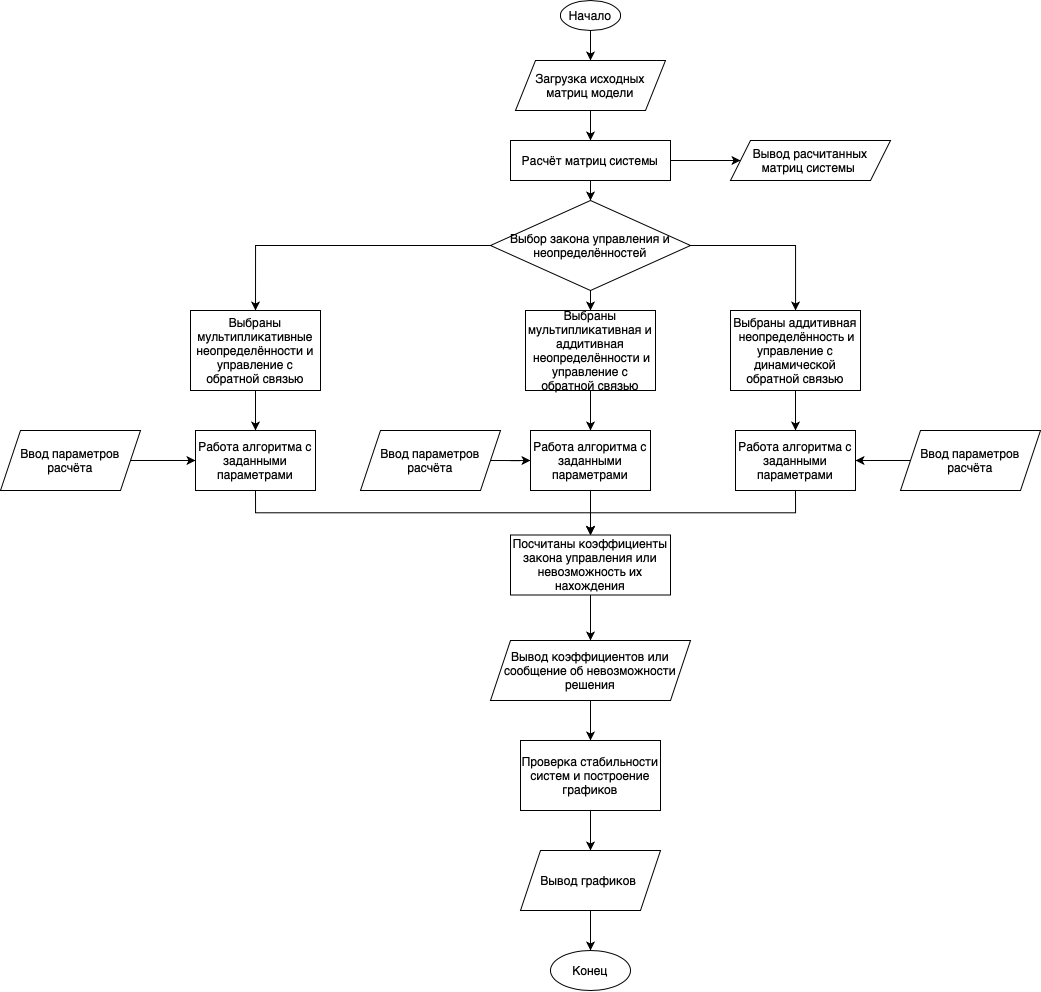
\includegraphics[scale=0.45]{images/programm.png}
	}
	\caption{Блок--схема программы с точки зрения пользователя}\label{fig:block}
\end{figure} 
\subsection{Описание робота}\label{sec:ch3/sect3/sub2}
В этом разделе мы численно подтверждаем приведённые ранее теоремы для нахождения оптимального робастного управления на примере реального четвероногого робота \textit{Unitree A1}, изображённого на Рисунке \cref{fig:unitree}.
\begin{figure}[ht]
	\centerfloat{
		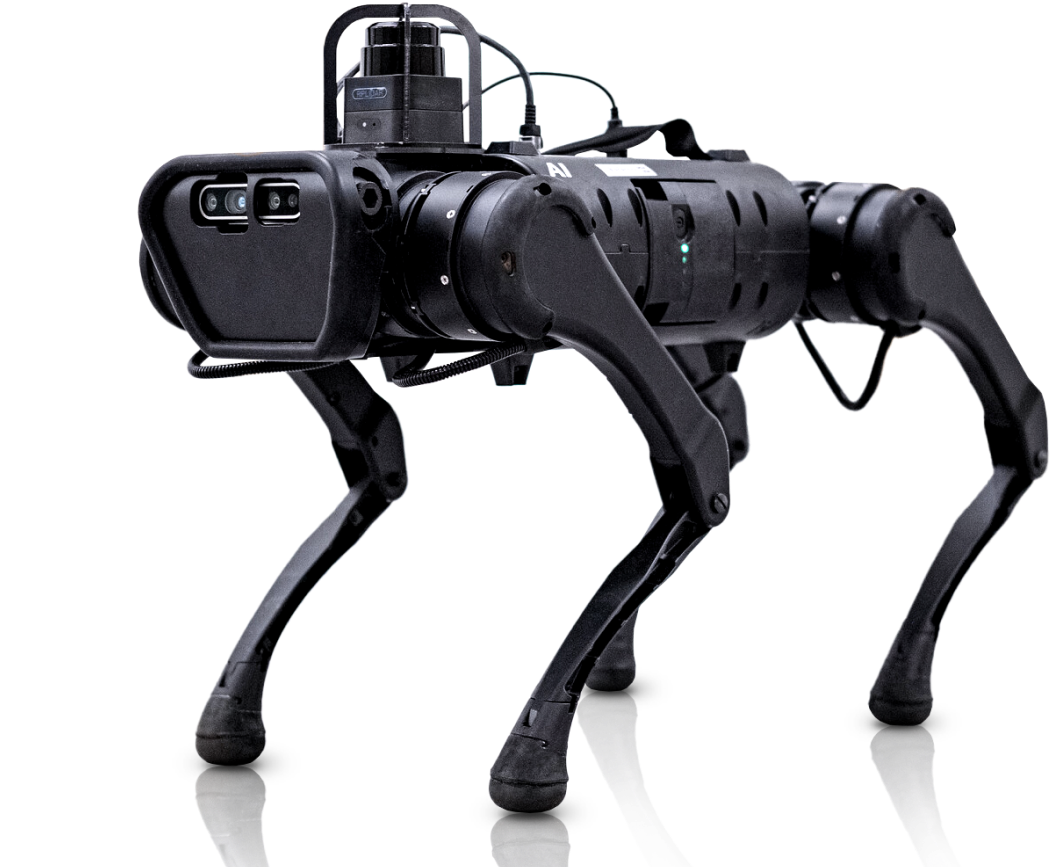
\includegraphics[scale=0.35]{images/unitree.png}
	}
	\caption{Unitree A1}\label{fig:unitree}
\end{figure} 

\begin{figure}[ht]
	\centerfloat{
		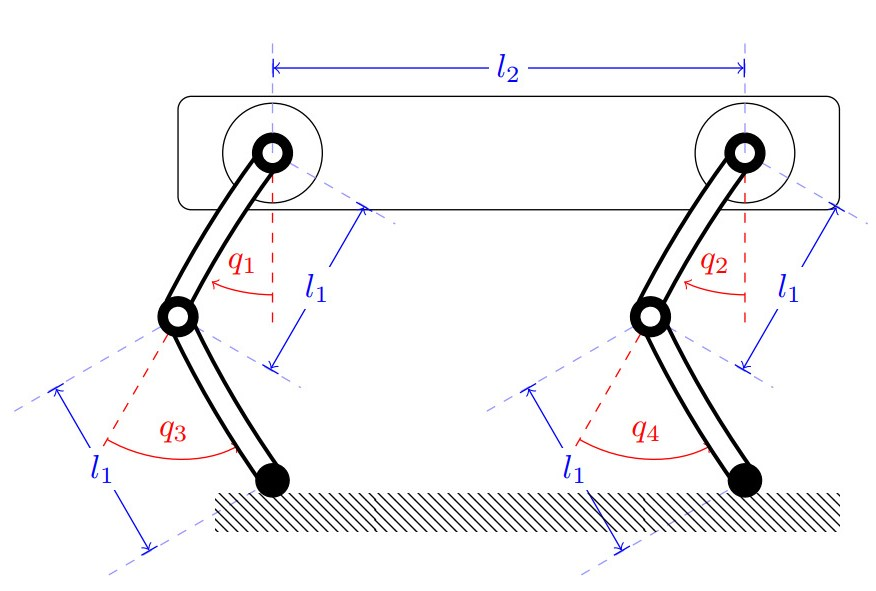
\includegraphics[scale=0.7]{images/FlatQuadruped.jpeg}
	}
	\caption{Схема плоского четвероногого робота}\label{fig:robotSagital}
\end{figure} 
Мы используем плоскую модель четвероногого робота (робот описывается в одном горизонтальном и одном вертикальном измерении), как показано на рисунке \ref{fig:robotSagital}, следуя \cite{RobotConfig}. Мы представляем его в виде пятизвенной структуры. Это позволяет нам описать положение робота с помощью семи обобщённых координат: положение и ориентация туловища робота и углы его четырёх суставов. Плоская модель объединяет ноги в пары --- конфигурация обеих передних ног описывается двумя одинаковыми координатами, то же самое справедливо и для обеих задних ног. 

Обозначим как $q_1$ и $q_2$ углы, связанные с суставами, соединяющими передние и задние ноги, соответственно, а $q_3$ и $q_4$ --- углы в коленных суставах передних и задних ног. Во время эксперимента ноги робота поддерживают контакт с землёй. Параметры робота, используемого в моделировании, приведены в Таблице \ref{tab:robotParam}.

\begin{table} [htbp]%
	\centering
	\caption{Параметры плоского четвероногого робота}%
	\label{tab:robotParam}% label всегда желательно идти после caption
	\renewcommand{\arraystretch}{1.5}%% Увеличение расстояния между рядами, для улучшения восприятия.
	\begin{SingleSpace}
		\begin{tabular}{@{}@{\extracolsep{20pt}}llll@{}} %Вертикальные полосы не используются принципиально, как и лишние горизонтальные (допускается по ГОСТ 2.105 пункт 4.4.5) % @{} позволяет прижиматься к краям
			\toprule     %%% верхняя линейка
			Звено & {Масса, кг} & {Длина, м} \\
			\midrule 
			Тело   & 10     & 0.5   \\
			Переднее бедро           & 2     & 0.3   \\
			Заднее бедро        & 2     & 0.3 \\
			Передняя голень        & 2     & 0.3 \\
			Задняя голень        & 2     & 0.3  \\
			\bottomrule %%% нижняя линейка
		\end{tabular}%
	\end{SingleSpace}
\end{table}

Моделирование построено следующим образом. Модель робота линеаризуется вдоль номинальной траектории, и для полученной линейной модели на каждом временном шаге путём решения уравнения Риккати находится стабилизирующий аффинный закон управления. Аналогичным образом на каждом временном шаге находятся коэффициенты усиления наблюдателя. Это представляет собой подход к планированию коэффициентов усиления при проектировании управления и наблюдателей \cite{Fromion2003}. Мы линеаризуем модель робота вокруг следующей конфигурации $q_1 =- \pi/6$, $q_2 = -\pi / 6$, $q_3 = \pi / 3$, и $q_4 = \pi / 3$.

\subsection{Численный эксперимент}\label{sec:ch3/sect3/sub3}
\nomenclature{ЗОУ}{Задача оптимизационного управления}
Продемонстрируем работу предложенного метода. Решим задачу оптимизационного управления (ЗОУ) \eqref{eq:thm3_OCP} для системы, описанной в предыдущем разделе с мультипликативными неопределённостями. Для параметра $\epsilon_1$ используется метод решётчатого поиска. 

\begin{figure}[ht]
	\centerfloat{
		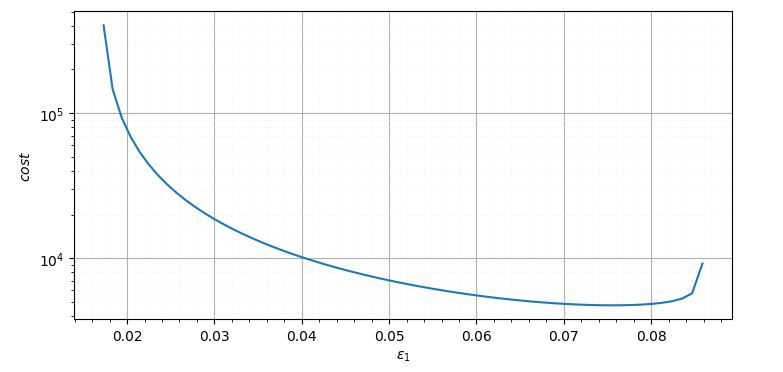
\includegraphics[scale=1.35]{images/mult_unitary_cost_eps.JPG}
	}
	\caption{Целевая функция для задачи оптимального управления \eqref{eq:thm3_OCP}, решённая для плоского четвероногого робота, построенная относительно параметра $\epsilon_1$; вертикальная ось масштабирована логарифмически, обе оси без единиц.}\label{fig:mult_unit_cost}
\end{figure} 

На рисунке~\ref{fig:mult_unit_cost} показано, как значение целевой функции зависит от $\epsilon_1$. Результаты показывают, что задача имеет решения, а значение целевой функции зависящее от $\epsilon_1$ описывается выпуклой кривой, что упрощает выбор оптимального значения этого параметра. 

Исходя из того, что зависимость значения целевой функции от $\epsilon_1$ является выпуклой, то мы можем найти такой параметр $\epsilon_1$, который будет давать минимальное значение целевой функции. В нашем эксперименте данным значением является $\epsilon_1 = 0.07535$. Для следующего графика сделаем этот параметр постоянным, для того чтобы продемонстрировать, что система стабилизируется для случайных неопределённостей. 

На рисунке \ref{fig:mult_unit_state} выведен вектор состояния для смоделированной системы на временном промежутке в \num{8} \si{\second}. На данном графике можно наблюдать, что система стабилизируется. На рисунке \ref{fig:mult_unit_state_hat} выведен вектор оценки состояния от времени, где можно также наблюдать, что система стабилизируется. 

\begin{figure}[ht]
	\centerfloat{
		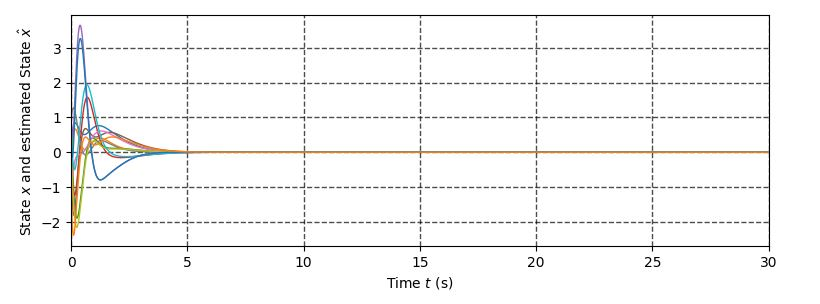
\includegraphics[scale=1.2]{images/mult_unit_state.JPG}
	}
	\caption{Вектор состояния от времени, при решении ЗОУ \eqref{eq:thm3_OCP} для плоского четвероногого робота, построенная относительно параметра $\epsilon_1$.}\label{fig:mult_unit_state}
\end{figure} 

\begin{figure}[ht]
	\centerfloat{
		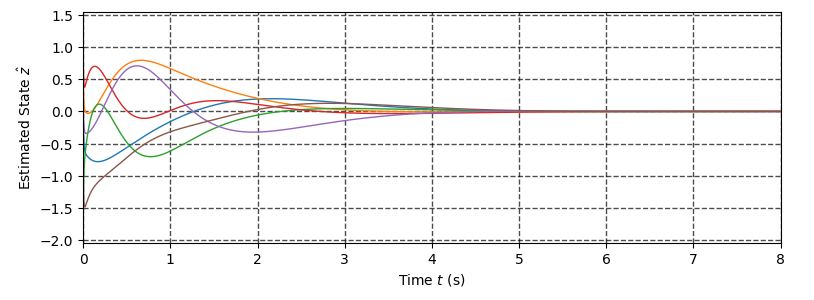
\includegraphics[scale=1.2]{images/mult_unit_state_hat.JPG}
	}
	\caption{Вектор оценки состояния от времени, при решении ЗОУ \eqref{eq:thm3_OCP} для плоского четвероногого робота, построенная относительно параметра $\epsilon_1$.}\label{fig:mult_unit_state_hat}
\end{figure} 

\begin{comment}

Рассмотрим следующую систему:
%
\begin{equation}
	\label{eq:part1_linear_dynamics}
	\begin{cases}
		\dot z=({A}_n+\Delta {A}_n)z + {A}_r\zeta + {B}u,\\
		y={C}{N}z+{C}{R}\zeta,
	\end{cases}
\end{equation}
%
где $z$ это динамические состояния, $\zeta = \text{const}$ - статические состояния и $\Delta {A}_n$ представляет мультипликативную модель неопределённостей и имеет следующую структуру:
%
\begin{equation}
	\label{eq:part1_uncertainty}
	\Delta {A}_n={M}_1{F}_1{N}_1 \quad \text{и} \quad {F}_1\T{F}_1\leq \nu {I},
\end{equation}
%
где ${M_1} \in \mathbb{R}^{n_z \times d}$ и 
${N_1} \in \mathbb{R}^{d \times n_z}$ известные матрицы, ${F}_1$ - неизвестная матрица ограниченная по норме и $\nu$ - неизвестный радиус - скаляр, определяющий лимит наложенный на норму ${F}_1$.

Следуя \cite{SAVIN2021} мы можем ввести наблюдатель Люнберга:
%
\begin{equation}
	\begin{bmatrix}
		\dot{\hat{z}} \\
		\dot{\hat{\zeta}}
	\end{bmatrix}=\begin{bmatrix}
		{A}_n & {A}_r \\
		0 & 0
	\end{bmatrix}
	\begin{bmatrix}
		\hat{z}\\ \hat{\zeta}
	\end{bmatrix}
	+  \begin{bmatrix}
		{B}\\0
	\end{bmatrix}u + {L} \left( y-\begin{bmatrix}
		{C}{N} & {C}{R}
	\end{bmatrix} \begin{bmatrix}
		\hat{z}\\ \hat{\zeta}
	\end{bmatrix} \right),
\end{equation}
%
где ${L}$ коэффициент наблюдателя.

Определим ошибку оценки состояния как $e = [ (z-\hat{z})\T \ \ (\zeta-\hat{\zeta})\T ]\T$ и введем блочную матрицу:
${S} = \begin{bmatrix}
	{I} \\ 0
\end{bmatrix}$, 
${E}=[ {N} \ \ {R}]$, и 
$
{A}_c=    \begin{bmatrix}
	{A}_r  & {A}_{\rho} \\
	0  & 0
\end{bmatrix}
$
записываем ошибку наблюдателя динамики:
%
\begin{equation}
	\label{eq:part1_error_dynamics}
	\dot e= ({A}_e-{L}{C}{E})e +{S}\Delta {A}_n z.
\end{equation}
%
Вводим закон управления:
%
\begin{equation}
	u={K}_z \hat{z}+{K}_{\zeta} \hat{\zeta},
\end{equation}
%
и определяем ${K}=\begin{bmatrix}
	{K}_z & {K}_{\zeta}
\end{bmatrix}$ записываем динамическую систему с обратной связью:
%
\begin{equation}
	\label{eq:part1_active_dynamics}
	\dot{z}=({A}_n+\Delta {A}_n +{B}{K}_z)z-{B}{K}e+({A}_r+{B}{K}_{\zeta})\zeta.
\end{equation}
%
Коэффициент регулятора ${K}_{\zeta}$ может быть выбран как:
%
\begin{equation}
	\label{eq:part1_static_control}
	{K}_{\zeta}=-{B}^{\dagger}{A}_r.
\end{equation}
%
Пока столбцы${A}_r$ лежат в подпространстве столбцов ${B}$ и существует точная оценка состояния, данный закон управления сводит на нет эффект $\zeta$ на динамику. В данном случае,отмечая что ${K}_z={K}{S}$,  мы можем представить ошибку наблюдателя и динамику робота как систему уравнений:
%
\begin{equation}
	\label{eq:part1_system}
	\begin{bmatrix}
		\dot{z} \\ \dot{e}
	\end{bmatrix}=\begin{bmatrix}
		({A}_n+\Delta {A}_n +{B}{K}{S}) & {B}{K} \\
		{S} \Delta {A}_n & ({A}_e-{L}{C}{E})        \end{bmatrix}\begin{bmatrix}
		z \\ e
	\end{bmatrix}.
\end{equation}
%
Рассмотрим проблему нахождения таких коэффициентов регулятора и наблюдателя, которые будут давать устойчивую систему для всех допустимых значений $\Delta {A}_n$.

\subsection{Единичная неопределённость}\label{sec:ch3/sect3/sub1}

Начнём с рассмотрения случая, когда неопределённость строго ограничена неравенством ${F}_1\T{F}_1\leq {I}$, которое мы называем единичной неопределённостью. В этом случае следующая теорема даёт нам достаточное условие устойчивости, которое может быть непосредственно использовано при проектировании регуляторов и коэффициентов усиления наблюдателей и представлено в виде линейного матричного неравенства с параметром.
\begin{theorem}\label{thm:part1_LMI_1}
	Система \eqref{eq:part1_system} асимптотически устойчива для всех матриц $\Delta {A}_n={M}_1{F}_1{N}_1$ с ${F}_1\T{F}_1\leq {I}$, если существуют положительно-определённые матрицы ${Q}_1>0$, ${P}_2>0$, матрицы $\hat{{K}}, \hat{{L}}$ и скаляры $\epsilon_1>0,\epsilon_2>0,\epsilon_3>0$ такие, что следующее линейное матричное неравенство выполнимо: 
	%
	\begin{equation}
		\label{eq:thm1_main_LMI}
		\begin{bmatrix}    
			{\Psi}_1  & 0 & {\Xi} & 0 &  {Q}_1{N}_1\T & {Q}_1{N}_1\T & 0\\
			* & {\Psi}_2 & 0 & {I} & 0 & 0 & {P}_2{S}{M}_1\\
			* & * &  -\frac{1}{\epsilon_1}{H} & 0 & 0 &0 & 0\\
			* & * & * & -\epsilon_1{H} & 0 & 0 & 0 \\
			* & * & * & * & -\epsilon_2 {I} & 0 & 0 \\       * & * & * & * & *& -\epsilon_3 {I} & 0 \\
			* & * & * & * & *& * & -\frac{1}{\epsilon_3} {I}
		\end{bmatrix} <0,
	\end{equation}
	%
	где
	%
	\begin{equation}
		\label{eq:H_Xi_variables}
		{H} = \begin{bmatrix}
			{Q}_1 & 0 \\
			0 & {I}
		\end{bmatrix}, \ \ 
		{\Xi} = \begin{bmatrix}
			{B}\hat{{K}} & {B}{K}_{\zeta} \end{bmatrix},
	\end{equation}
	%
	\begin{align}
		\label{eq:Psi_1}
		{\Psi}_1&={Q}_1{A}_n\T+{A}_n{Q}_1+{B}\hat{{K}}+\hat{{K}}\T{B}\T  +\epsilon_2{M}_1{M}_1\T, \\
		\label{eq:Psi_2}
		{\Psi}_2 &={A}_e\T{P}_2+{P}_2{A}_e-\hat{{L}}{CE}-{E}\T{C}\T\hat{{L}}\T,
	\end{align}
	%
	и коэффициенты регулятора и наблюдателя находятся как ${L}={P}^{-1}_2\hat{{L}}$
	и ${KS}=\hat{{K}}{Q}^{-1}_1$.  
\end{theorem}
\begin{proof}
	Введём переменную ${\vartheta}=[
	z\T \ e\T ]\T$ и напишем кандидата в функцию Ляпунова: 
	%
	\begin{equation}
		V
		=
		\begin{bmatrix}
			z \\ e
		\end{bmatrix}\T
		\begin{bmatrix}
			{P}_1 & 0 \\
			0 & {P}_2
		\end{bmatrix}
		\begin{bmatrix}
			z  \\ e
		\end{bmatrix}
		=
		\vartheta\T{P}\vartheta
		>0.
	\end{equation}
	%
	Производная по времени от функции-кандидата Ляпунова представляет собой квадратичную форму, которая должна быть отрицательно-определённой. Это можно записать в виде следующего матричного неравенства:
	\begin{equation}
		\label{eq:matrix_Young}
		\begin{bmatrix}
			{\Sigma}_1+{P}_1\Delta {A}_n+ (\Delta {A}_n)\T {P}_1 & ({S} \Delta {A}_n)\T{P}_2 -{P}_1{BK} \\
			{P}_2{S}\Delta {A}_n - ({BK})\T{P}_1 & {\Sigma}_2
		\end{bmatrix}<0,
	\end{equation}
	%
	где
	%
	\begin{align}
		{\Sigma}_1&= {P}_1({A}_n+{BKS})+({A}_n+{BKS}){P}_1\T, \\  
		{\Sigma}_2&={P}_2({A}_e-{LCE})+({A}_e-{LCE})\T{P}_2.
	\end{align}
	%
	Теперь, подставив \eqref{eq:part1_uncertainty} в \eqref{eq:matrix_Young} и сопрягая по $diag({Q}_1, {I})$, получим:
	\begin{equation}
		\label{eq:Young_conjugated}
		\begin{bmatrix}
			{\Pi}_1+{M}_1{F}_1{N}_1{Q}_1 + {Q}_1({M}_1{F}_1{N}_1)\T   & {Q}_1({S} {M}_1{F}_1{N}_1)\T{P}_2 -{BK} \\
			{P}_2{M}_1{F}_1{N}_1{Q}_1 - ({BK})\T & {\Sigma}_2
		\end{bmatrix} <0,
	\end{equation}
	%
	где $ {\Pi}_1=({A}_n+{BKS}){Q}_1+{Q}_1({A}_n+{BKS})\T$ и ${Q}_1 ={P}_1^{-1}$.
	Используя лемму \ref{lemma:Young} уравнения \eqref{eq:Young_relation_BMI} и \eqref{eq:Young_robust_2} с $\nu=1$ мы расширяем последнее выражение следующим образом (см. приложение \ref{apx:A}):
	\begin{equation}
		\label{eq:thm1_LMI_after_Young}
		\begin{bmatrix}
			{\Gamma}_1  & 0  \\
			0 & {\Sigma}_2 +\frac{1}{\epsilon_1}{H}^{-1} +\epsilon_3 {P}_2{S}{M}_1({P}_2{S}{M}_1)\T
		\end{bmatrix}<0,
	\end{equation}
	%
	где
	%
	\begin{equation}
		\label{eq:thm1_pre_final_LMI_Gamma}
		{\Gamma}_1={\Pi}_1 +\epsilon_1{BKH}{K}\T{B}\T+ \left(\frac{1}{\epsilon_2}+\frac{1}{\epsilon_3} \right){Q}_1{N}_1\T{N}_1{Q}_1 + \epsilon_2 {M}_1{M}_1\T.
	\end{equation}
	%
	Применяя дополнение Шура \ref{lemma:Schur}:
	%
	\begin{equation}
		\label{eq:thm1_pre_final_LMI}
		\begin{bmatrix}
			{\Pi}_1 +\epsilon_2{M}_1{M}_1\T & 0 & {BKH} & 0 &  {Q}_1{N}_1\T & {Q}_1{N}_1\T & 0\\
			* & {\Sigma}_2 & 0 & {I} & 0 & 0 & {P}_2{S}{M}_1\\
			* & * &  -\frac{1}{\epsilon_1}{H} & 0 & 0 &0 & 0\\
			* & * & * & -\epsilon_1{H} & 0 & 0 & 0 \\
			* & * & * & * & -\epsilon_2 {I} & 0 & 0 \\       * & * & * & * & *& -\epsilon_3 {I} & 0 \\
			* & * & * & * & *& * & -\frac{1}{\epsilon_3} {I}\\
		\end{bmatrix} <0.
	\end{equation}
	%
	Замена переменных $\hat{{L}}={P}_2{L}$ и $\hat{{K}}={KS}{Q}_1$
	показывает нам эквивалентности ${\Psi}_1={\Pi}_1+\epsilon_2{M}_1{M}_1\T$ , ${\Psi}_2={\Sigma}_2$ и ${BKH}={\Xi}$; и подставляет их в \eqref{eq:thm1_pre_final_LMI}, находим окончательное линейное матричное неравенство \eqref{eq:thm1_main_LMI}, 
	где ${\Psi}_1$ и ${\Psi}_2$ определяются как выражения \eqref{eq:Psi_1} и \eqref{eq:Psi_2}.
	Это линейное матричное неравенство с переменными ${Q}_1,{P}_2, \hat{{K}},\hat{{L}}$ и $\epsilon_2$. Скаляры $\epsilon_1$ и $\epsilon_3$ постоянные параметры, которые должны быть выбраны перед решением проблемы.
Подставляя \ref{rmk:alpha_beta} в \eqref{eq:thm1_main_LMI} и применяя дополнение Шура, мы получаем линейно матричное неравенство в переменных 
${Q}_1$, ${P}_2$, $\hat{{K}}$, $\hat{{L}}$, $\epsilon_2$, $\alpha$, и $\beta$.
%
\begin{equation}
	\label{eq:thm1_final_LMI_ab}
	\begin{bmatrix}    
		{\Psi}_1  & 0 & {\Xi} & 0 &  {P}_1{N}_1\T & {Q}_1{N}_1\T & 0 & 0 & 0\\
		* & {\Psi}_2 & 0 & {I} & 0 & 0 & {P}_2{S}{M}_1 & 0 & 0\\
		* & * &  -\frac{1}{\epsilon_1}{H} & 0 & 0 &0 & 0& 0 & 0\\
		* & * & * & -\epsilon_1{H} & 0 & 0 & 0 & 0 & 0 \\
		* & * & * & * & -\epsilon_2 {I} & 0 & 0 & 0 & 0 \\       * & * & * & * & *&  -2\alpha {I} & 0 & \beta {I} &0 \\
		* & * & * & * & *& * & -2\beta {I} & 0 & \alpha {I} \\
		* & * & * & * & *&*&* &-{I}&0\\
		* & * & * & * & *&*&*&* &-{I}
	\end{bmatrix} <0.
\end{equation}
\end{proof}

Используя теорему \ref{thm:part1_LMI_1} и добавляя выпуклую целевую функцию, мы формулируем робастную конструкцию управления в виде полуопределённой программы:
%
\begin{equation}
	\label{eq:thm1_OCP}
	\begin{aligned}
		& \underset{\epsilon_2,\alpha,\beta, {Q}_1, {P}_2,\hat{{K}} , \hat{{L}} }{\text{minimize}}
		& & \operatorname{tr}({Q}_1\T{W}_z{Q}_1)+ \operatorname{tr}({P}_2\T{W}_e{P}_2)+ \operatorname{tr}(\hat{{K}}\T{W}_k\hat{{K}})+\operatorname{tr}(\hat{{L}}\T{W}_l\hat{{L}}), \\
		& \text{subject to}
		& & \begin{cases}
			{Q}_1>0, \ \
			{P}_2>0, \ \
			\epsilon_2>0, \ \
			\alpha>0, \ \
			\beta>0, \\
			\text{условие \eqref{eq:thm1_final_LMI_ab} },
		\end{cases}
	\end{aligned}
\end{equation}
где ${W}_z,{W}_e,{W}_k$ и ${W}_l$ - весовые матрицы. 
\subsection{Мягкая неопределённость}\label{sec:ch3/sect3/sub2}
Пусть матрица неопределённости $\Delta {A}_n$ определяется как:
%
\begin{equation}
	\label{eq:nu_uncertainty}
	\Delta {A}_n={M}_1{F}_1{N}_1 \quad \text{и} \quad {F}_1\T{F}_1\leq \nu {I}.
\end{equation}
%
Мы можем предложить условия на усиление регулятора и наблюдателя, которые гарантируют устойчивость при любом допустимом значении ${F}_1$ для заданного радиуса неопределённости $\nu$:
%
\begin{theorem}\label{thm:part1_LMI_2}
	Система \eqref{eq:part1_system}
	асимптотически устойчива для любой $\Delta {A}_n =$${M}_1{F}_1{N}_1$ с ${F}_1\T{F}_1\leq \nu {I}$, если существуют положительно-определённые матрицы ${Q}_1>0$, ${P}_2>0$, матрицы $\hat{{K}}, \hat{{L}}$ и скаляр $\bar{\epsilon}>0$ такие, что следующее линейное матричное неравенство выполнимо: 
	%
	\begin{equation}
		\label{eq:thm2_final_LMI}
		\begin{bmatrix}    
			{\Upsilon}_1  & 0 & {\Xi} & 0 &  {Q}_1{N}_1\T & {M}_1 & 0\\
			* & {\Psi}_2 & 0 & {I} & 0 & 0 & {P}_2{S}{M}_1\\
			* & * &  -\frac{1}{\epsilon_1}{H} & 0 & 0 &0 & 0\\
			* & * & * & -\epsilon_1{H} & 0 & 0 & 0 \\
			* & * & * & * & -\frac{\bar{\epsilon}}{2}{I} & 0 & 0 \\       * & * & * & * & *&  -\bar{\epsilon}{I} & 0 \\
			* & * & * & * & *& * &  -\bar{\epsilon}{I}
		\end{bmatrix} <0,
	\end{equation}
	%
	где
	%
	\begin{equation}
		\label{eq:Upsilon_1}
		{\Upsilon}_1={Q}_1{A}_n\T+{A}_n{Q}_1+{B}\hat{{K}}+\hat{{K}}\T{B}\T, 
	\end{equation}
	Матрицы ${\Psi}_2$, ${\Xi}$ те же, что и в уравнениях \eqref{eq:Psi_2},\eqref{eq:H_Xi_variables},
	а коэффициенты регулятора и наблюдателя задаются ${L}={P}^{-1}_2\hat{{L}}$.
	и ${KS}=\hat{{K}}{Q}^{-1}_1$.
\end{theorem}
\begin{proof}
	Первая часть доказательства совпадает с доказательством теоремы \ref{thm:part1_LMI_1} (до уравнения \eqref{eq:Young_conjugated}). Используя уравнения \eqref{eq:Young_relation_BMI} и \eqref{eq:updated_Young_robust_2} из леммы \ref{lemma:Young}, получаем
	%
	\begin{equation}
		\label{eq:thm2_LMI_after_Young}
		\begin{bmatrix}
			{\Phi}  & 0  \\
			0 & {\Sigma}_2 +\frac{1}{\epsilon_1}{H}^{-1} +\epsilon {P}_2{S}{M}_1({P}_2{S}{M}_1)\T
		\end{bmatrix}<0,
	\end{equation}
	%
	где $\epsilon=\sqrt{\nu}>0$ и
	%
	\begin{equation}
		{\Phi}={\Sigma}_1 
		+\epsilon_1{BKH}{K}\T{B}\T+ 2\epsilon {Q}_1{N}_1\T{N}_1{Q}_1 + \epsilon {M}_1{M}_1\T.
	\end{equation}
	%
	Используя дополнение Шура, преобразуем это условие в: 
	%
	\begin{equation}
		\label{eq:thm2_pre_final_LMI}
		\begin{bmatrix}
			{\Sigma}_1  & 0 & {BKH} & 0 &  {Q}_1{N}_1\T & {M}_1 & 0\\
			* & {\Sigma}_2 & 0 & {I} & 0 & 0 & {P}_2{S}{M}_1\\
			* & * &  -\frac{1}{\epsilon_1}{H} & 0 & 0 &0 & 0\\
			* & * & * & -\epsilon_1{H} & 0 & 0 & 0 \\
			* & * & * & * & -\frac{\bar{\epsilon}}{2}{I} & 0 & 0 \\       * & * & * & * & *& -\bar{\epsilon} {I} & 0 \\
			* & * & * & * & *& * & -\bar{\epsilon} {I}\\
		\end{bmatrix} <0,
	\end{equation}
	%
	где $\bar{\epsilon}=\frac{1}{\epsilon}$, и, наконец, используя замену переменных 
	$\hat{{L}}={P}_2{L}$ и $\hat{{K}}={KS}{Q}_1$
	находим, что ${\Upsilon}_1={\Sigma}_1$, ${\Psi}_2={\Sigma}_2$ и ${BKH}={\Xi}$ и, подставляя в \eqref{eq:thm2_pre_final_LMI}, находим окончательное линейное матричное неравенство \eqref{eq:thm2_final_LMI}. 
\end{proof}
Это неравенство в переменных ${Q}_1,{P}_2,\hat{{K}} , \hat{{L}},\bar{\epsilon}$.
Мы можем выполнить поиск $\epsilon_1$, как описано в примечании \ref{rm:griding_search}. 

В качестве целевой функции мы можем использовать минимизацию $\bar{\epsilon}$, что эквивалентно максимизации $\nu$, так как $\nu=\frac{1}{\bar{\epsilon}^2}$. Тогда задача оптимизации приобретает вид:
%
\begin{equation}
	\label{eq:thm2_OCP}
	\begin{aligned}
		& \underset{\bar{\epsilon},{Q}_1, {P}_2,\hat{{K}} , \hat{{L}} }{\text{minimize}}
		& &  \bar{\epsilon}, \\
		& \text{subject to}
		& & \begin{cases}
			{Q}_1>0, \ \
			{P}_2>0, \ \
			\bar{\epsilon}>0, \\
			\text{condition \eqref{eq:thm2_final_LMI} }.
		\end{cases}
	\end{aligned}
\end{equation}
\end{comment}

\clearpage
